%%
%% Copyright 2007, 2008, 2009 Elsevier Ltd
%%
%% This file is part of the 'Elsarticle Bundle'.
%% ---------------------------------------------
%%
%% It may be distributed under the conditions of the LaTeX Project Public
%% License, either version 1.2 of this license or (at your option) any
%% later version.  The latest version of this license is in
%%    http://www.latex-project.org/lppl.txt
%% and version 1.2 or later is part of all distributions of LaTeX
%% version 1999/12/01 or later.
%%
%% The list of all files belonging to the 'Elsarticle Bundle' is
%% given in the file `manifest.txt'.
%%
%% Template article for Elsevier's document class `elsarticle'
%% with harvard style bibliographic references
%% SP 2008/03/01

\documentclass[final,3p,times,twocolumn]{elsarticle}

%% Use the option review to obtain double line spacing
%% \documentclass[authoryear,preprint,review,12pt]{elsarticle}

%% Use the options 1p,twocolumn; 3p; 3p,twocolumn; 5p; or 5p,twocolumn
%% for a journal layout:
%% \documentclass[final,1p,times]{elsarticle}
%% \documentclass[final,1p,times,twocolumn]{elsarticle}
%% \documentclass[final,3p,times]{elsarticle}
%% \documentclass[final,3p,times,twocolumn]{elsarticle}
%% \documentclass[final,5p,times]{elsarticle}
%% \documentclass[final,5p,times,twocolumn]{elsarticle}

%% For including figures, graphicx.sty has been loaded in
%% elsarticle.cls. If you prefer to use the old commands
%% please give \usepackage{epsfig}

%% The amssymb package provides various useful mathematical symbols
\usepackage{amssymb}
\usepackage{epstopdf}
\usepackage{hyperref}
\usepackage{color}

%% The amsthm package provides extended theorem environments
%% \usepackage{amsthm}

%% The lineno packages adds line numbers. Start line numbering with
%% \begin{linenumbers}, end it with \end{linenumbers}. Or switch it on
%% for the whole article with \linenumbers.
%% \usepackage{lineno}

\journal{Applied Acoustics}

\newcommand{\ml}[1]{\textcolor{blue}{ Mathieu: #1}}


\begin{document}

\begin{frontmatter}

%% Title, authors and addresses

%% use the tnoteref command within \title for footnotes;
%% use the tnotetext command for theassociated footnote;
%% use the fnref command within \author or \address for footnotes;
%% use the fntext command for theassociated footnote;
%% use the corref command within \author for corresponding author footnotes;
%% use the cortext command for theassociated footnote;
%% use the ead command for the email address,
%% and the form \ead[url] for the home page:
%% \title{Title\tnoteref{label1}}
%% \tnotetext[label1]{}
%% \author{Name\corref{cor1}\fnref{label2}}
%% \ead{email address}
%% \ead[url]{home page}
%% \fntext[label2]{}
%% \cortext[cor1]{}
%% \address{Address\fnref{label3}}
%% \fntext[label3]{}


\title{An efficient audio coding scheme for large scale acoustic monitoring}

%% use optional labels to link authors explicitly to addresses:
%% \author[label1,label2]{}
%% \address[label1]{}
%% \address[label2]{}

\author{Felix Gontier, Mathieu Lagrange, Arnaud Can, Catherine Lavandier}

\address{felix.gontier@reseau.eseo.fr\\mathieu.lagrange@cnrs.fr}

\begin{abstract}
%% Text of abstract
The advent of low cost acoustic sensors together with the need to better monitor and comprehend the acoustic environment of urban and wilderness areas give rise to the deployment of experimental sensor networks such as the sonyc (wp.nyu.edu/sonyc) and cense (cense.ifsttar.fr) projects.

Together with the estimation of acoustic indicators (LAeq, ...), one important aspect of those networks is their ability to detect the presence of sound sources of interest ( bird calls, sirens, explosion, ...) in order to better assess soundscapes. This detection step can be operated online (on the sensors) or offline (on the data servers).

The former is efficient in terms of data storage as only the detection events are transmitted. Though, it requires the availability of computing resources on the sensors in order to perform the detection step, and the detection is done once and cannot be recomputed.

The latter scheme has several benefits. First, the sensor is much simpler and can thus be autonomous in terms of energy, easing the deployment of the network. Second, it allows researchers to gather large amount of data that can be post processed and studied further offline. Data can be re analysed following newer classification schemes or using new indicators.

But, for transmission from the sensors to the storage unit, the data needs to be encoded in an efficient way. Also, as the data is transmitted using the network and stored, one must ensure that the intelligibility of potential speech utterances is lost during the coding process, in order to ensure the privacy of the citizens.

The coding scheme described in this paper has the following features. It is of low bitrate but still allows the computation of most of the standard acoustics indicators with high precision. As far as acoustic event detection is concerned, we report equivalent performance of several state of the art classification schemes from features computed using raw audio data and encoded data. Finally, according to preliminary perceptual evaluation, the proposed coding scheme very strongly degrades the intelligibility, thus ensuring citizen privacy.

In order to promote reproducible research, the coder as well as the experiments needed to generate the figures will be made available to the community.



\end{abstract}

\begin{keyword}
%% keywords here, in the form: keyword \sep keyword

%% PACS codes here, in the form: \PACS code \sep code

%% MSC codes here, in the form: \MSC code \sep code
%% or \MSC[2008] code \sep code (2000 is the default)

\end{keyword}

\end{frontmatter}

%% \linenumbers
\clearpage
%% main text
\section{Introduction}
%\label{}

\section{Background}

\ml{decrit ici les besoins avec une biblio}

\subsection{acoustic monitoring}

db spl, tiers d'octave, etc

10 refs

et dire que a partir de tiers d'ocatve 125 on peut retrouver tout les autres

\subsection{event detection}

15 refs

\section{Encoding scheme}

As audio signals in the time domain offers very few, often inefficient processing possibilities to reduce data size, a common practice is to prefer the frequency domain which in many cases provides a better information representation. Therefore, we first apply a short-term Fourier transform (STFT) to the arbitrary-length signal (sampled continously in our application). The phase is then discarded, being mostly retrievable under certain conditions \cite{nawab1983}, as well as resulting negative frequency components which are redundant due to the real nature of studied signals. However, these operations do not induce a significant gain in data size compared to the raw audio. A solution is the implementation of auditory filterbanks to concentrate relevant information into a fixed number of values in the same way the human cochlea does, that is, grouping frequency coefficients around critical bands in a logarithmic scale. This technique offers an important advantage beyond the information-dimensionality ratio improvement: in the Fourier squared magnitude domain, it only amounts to a single matrix multiplication which can be reversed to some degree. In this work, we study two different filterbanks and propose a set of analysis parameters for each.\\

\ml{ce n'est pas vraiment ca. On a une contrainte qui est que l'on veut coder des données utilissables pour le monitoring acoustique et la reco d'evenements qui considère des représentations spécifiques. Je te propose donc de passer en revue les deux côtés dans la section ci dessus (background) et dire que nos choix sont raisonnables.}

We first use the widely known Mel scale as implemented by the \textit{rastamat} library \cite{ellis2005}. STFT analysis frames are obtained by applying a Hann window on 23.2~ms of signal with 50\% (11.6~ms) overlap to allow for phase recovery.\\

Another studied auditory transformation is the calculation of third-octave bands, generally used to compute the equivalent sound level $L_{eq}$ when acoustic measurements are needed. While the related filters are usually applied in the time domain, \cite{antoni2010} presents a frequency weights matrix design procedure that complies with both ANSI S1.1-1986 and IEC 61260-1:2014 standards, while respecting the partition of unity principle over all frequency bins in the relevant range. We implement this method for third-octave bands -17 to 13, ie. 20~Hz - 20kHz range, although with a minor change: inverting the use of sines and cosines is found to be a more intuitively correct approach, as we believe was the author's original intention. The STFT is computed for 125~ms audio windows, zero-padded to maximize FFT performance after the application of a rectangular function. No overlap is used to maximize the efficiency of the process as it is not needed to match the concept of "fast" acoustical measurements (8 per second). The rectangular window choice is made to ensure energy conservation in a given analysis frame. Results are compared with Couvreur's implementation \cite{couvreur}. We observe similar results and a better handling of sidemost bands: low frequencies where resolution is poor and higher frequencies where cutoff frequencies are superior than Nyquist's frequency rendering most time-domain filter designs difficult. \ml{pas clair}

\ml{mettre des chiffres ou une figure pour motiver ton choix dans la section dédiée et faire ici une ref}

\subsection{Data Encoding}

\ml{en general tes phrases sont trop longues. Coupe en deux des que tu peux et pas de paranthèses !!}

A Huffman coding scheme \cite{} is then used to further reduce data dimensionality. As in most entropy coding algorithms, the efficiency of this technique depends on two important factors: a reduced amount of symbols \ml{in the dictionnary ?} and a low data entropy \ml{explique ce dernier point}. The first is generally obtained by applying a quantization process to the signal, whereas the second is directly linked with the probability density function (PDF) of these symbols, with entropy decreasing when very few symbols have a very high probability of appearance. Considering an estimated PDF for our data as shown in Figure~\ref{fig:pdf}a, immediately applying a linear quantization clearly results in most of the information being lost. We therefore spread the PDF by taking the logarithm (natural or base 10) of the signal, then apply a linear quantization with $2^{q-1}-1$ output values to obtain Figure~\ref{fig:pdf}b. Finally, we use a $\Delta$-encoding algorithm \cite{} along the time dimension to reduce redundancies and effectively concentrate higher probabilities on symbols around zero (Figure~\ref{fig:pdf}c). This yields a higher amount of symbols at $2^q-1$ but a nevertheless smaller entropy. In the example shown here, the former is $H_{log} = 6.24~sh$ and the latter $H_{\Delta} = 3.54~sh$. Huffman encoding is then computed for texture frames of several minutes with a frame-specific symbol-code dictionnary. Indeed, we found that using a single dictionnary generated with an entire dataset was not beneficial in terms of efficiency or computation time. Alternatively, analysis frames can be encoded and sent separately for continous transfers using one general dictionnary.

\ml{a discuter. Pourquoi ne pas avoir un dic fixe, ce doit etre couteux de faire huffman a chaque fois ?}

\ml{ici encore, il faut mettre des chiffres pour motiver ce choix. plutot faire des refs a la subsection dediée}

\begin{figure*}[htbp]
	\centering
		\includegraphics[width=0.8\textwidth]{pdf.eps}
	\caption{Example of estimated probability density functions of the data throughout the encoding step. (left) Unchanged output of the representation step, concentrated towards very low values. (middle) PSD "flattening" effect induced by logarithm application. Here values are mapped to the range $[0, 2^7-1]$ and rounded to perform quantization. (right) Output of the $\Delta$ compression, with desirable probabilities as the input to a Huffman algorithm.}
	\label{fig:pdf}
\end{figure*}
6.24 before
3.54 after

The decoding process is quite straightforward, as both Huffman and $\Delta$ compression are lossless and directly reversible.


The entire coder process is summarized in Figure~\ref{fig:scheme}.

\begin{figure*}[htbp]
	\centering
		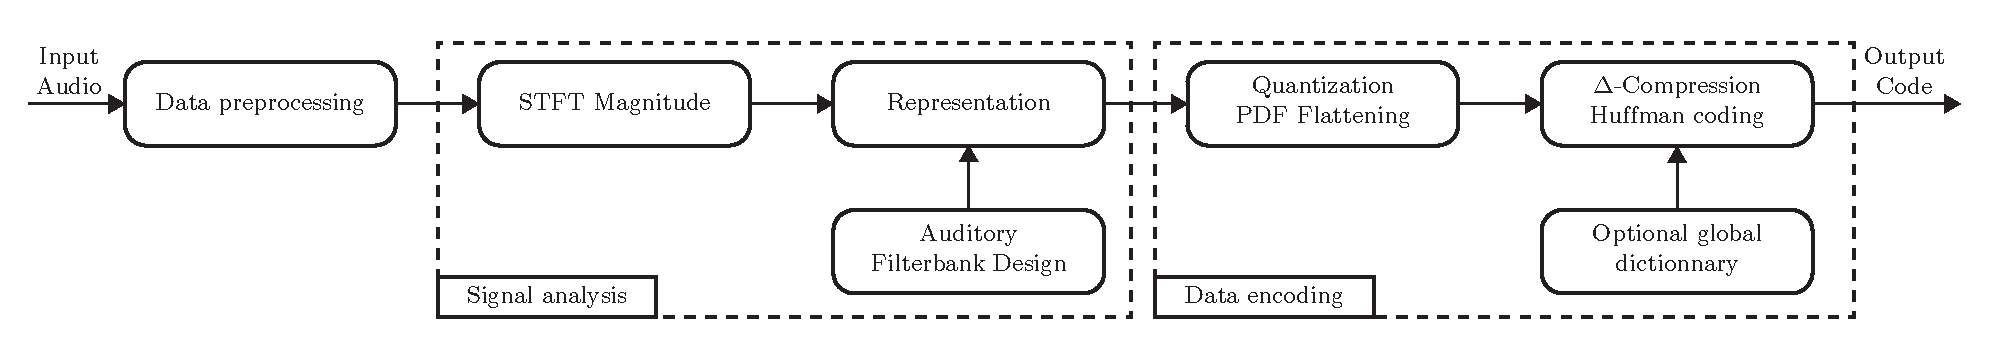
\includegraphics[width=1\textwidth]{scheme.pdf}
	\caption{Overview of the coder process.}
	\label{fig:scheme}
\end{figure*}

\section{Evaluation}
A set of metrics is computed to assess the efficiency of the proposed coder scheme and determine the impact of the algorithm's parameters, which are as follow: the desired word size prior to Huffman encoding, set by quantization for both signal representation choices, and only for Mel bands the number of coefficients between 10 and 40. We also study the effect of time averaging analysis frames: to force a fixed amount of frames per second lesser than the average speech rate in phonemes per second is a possible way to alter intelligibility at the cost of temporal information resolution.\\

\subsection{efficiency}

detaille les resulats pour l'efficacité de codage


\subsection{recognition}


The UrbanSound8k dataset\cite{salamon2014} features about 9 hours of urban environmental sounds recordings separated in 8732 wave files ranging from 1 to 4 seconds each. The recordings are labeled in 10 classes (air conditioner, car horn, children playing, dog bark, drilling, enginge idling, gun shot, jackhammer, siren, street music), and distributed in 10 independant folds. A method and baseline results are also provided for the classification task. It is used in all the following experiments with the exception of intelligibility computation for which a small dataset of high-quality voice recordings is preferred. Audio files are resampled 44.1 samples per second, normalized and reduced to a single channel.\\

We first evaluate the global loss of information by implementing the four classification models proposed in \cite{salamon2014}: a support vector machine with a radial basis function kernel, a random forest classifier with 500 trees, a decision tree and a k-nearest neighbors classifier with $k = 5$. Values for the SVM parameter $C$ and RBF kernel variance $\sigma^2$ are found with a grid search. We apply a discrete cosine transform to the critical band signal representation to obtain cepstra (known as Mel Frequency Cepstrum Coefficients or MFCC in the first case) of which we conserve the 25 first coefficients, and summarize along time with the mean, variance, skewness, kurtosis, minimum, maximum, median, derivative mean and variance, second order derivative mean and variance. The feature vector is thus comprised of 275 values to reproduce available results and compare with our own. Models are trained for each setup using the 10-fold method, that is, every combination of testing one fold on models trained with the other nine.\\

\subsection{Inintelligibility}

Intelligibility in decoded and reconstructed audio is also one of the main concerns of this study. We conduct preliminary perceptive tests to ensure that a clean speech recording is made unintelligible, implying the same results in usually noisier urban soundscapes. We also provide the computation of two objective metrics: the Coherence Speech Intelligibility Index\cite{kates2005} (CSII) and frequency-eighted segmental SNR\cite{hu2008} (fwSNRseg) by comparing original unaltered samples and recovered audio. These two indicators have been shown to correlate well with perceptual tests\cite{ma2009}, although results are only available for lesser degradations and distortions.\\

	\ml{j'ai mis le paragraphe en dessous pour des raisons de clarté car cela ne fait pas parti du codeur. A reformuler}

 Recovering a linearly-scaled spectrogram can be achieved by scaling the transpose of the forward transformation matrix, although a loss of resolution increasing with frequency is induced due to the shape of the transformation, as illustrated by Figure~\ref{fig:freq}. Signal phase is approximated by either white noise spectrogram scaling or a Griffin\& Lim algorithm \cite{griffin1984}, and the signal is retrieved using overlap-add. When using overlap while computing third-octave bands, one can also avoid framing effects produced by rectangular windowing by convoluting the signal with another windowing function prior to inverse-STFT computation.\\

\begin{figure}[htbp]
	\centering
		\includegraphics[width=\columnwidth]{freq.png}
	\caption{Third-octave bands analysis and approximate inverse transformation effects on energy location. This process yields an important and heterogeneous loss in resolution, particularly at higher frequency points.}
	\label{fig:freq}
\end{figure}


The coder's output bitrate as well as additional measurement error is computed for both data representations, it is expressed in dB and compared to the IEC 61672-1:2013 standard on sound level meter tolerance. This is to verify that the quantization step yields a maximum absolute error inferior to the precision of the recording device. To provide relevant statistics, these quantities are estimated for a total of 53 10-minutes texture frames.\\

\section{Results}

\section{Conclusion}

\clearpage
%% The Appendices part is started with the command \appendix;
%% appendix sections are then done as normal sections
%% \appendix

%% \section{}
%% \label{}

%% If you have bibdatabase file and want bibtex to generate the
%% bibitems, please use
%%
%%  \bibliographystyle{elsarticle-harv}
%%  \bibliography{<your bibdatabase>}

%% else use the following coding to input the bibitems directly in the
%% TeX file.
\section{References}
\begin{thebibliography}{09}

\bibitem{nawab1983}
Nawab, H. and Quatieri, T. and Lim, J. (1983). Signal reconstruction from short-time Fourier transform magnitude. \textit{IEEE Transactions on Acoustics, Speech, and Signal Processing}, 31(4)

\bibitem{ellis2005}
Ellis, D. (2005). \textit{{PLP} and {RASTA} (and {MFCC}, and inversion) in {M}atlab}. Available at: \url{http://www.ee.columbia.edu/~dpwe/resources/matlab/rastamat/}

\bibitem{antoni2010}
Antoni, J. (2010). Orthogonal-like fractional-octave-band filters. \textit{J. Ac. Soc. Am.}, 127(2)

\bibitem{couvreur}
Couvreur, C. \textit{Implementation of a one-third-octave filter bank in Matlab}. Available at: \url{http://citeseer.ist.psu.edu/24150.html}

\bibitem{griffin1984}
Griffin, D. and Lim, J. (1984). Signal Estimation from Modified Short-Time Fourier Transform. \textit{IEEE Transactions on Acoustics, Speech, and Signal Processing}, 32(2)

\bibitem{salamon2014}
Salamon, J. and Jacoby, C. and Bello, J. (2014). A Dataset and Taxonomy for Urban Sound Research. \textit{Proceedings of the 22nd ACM international conference on Multimedia}

\bibitem{kates2005}
Kates, J. and Arehart, K. (2005). Coherence and the Speech Intelligibility Index. \textit{J. Ac. Soc. Am.}, 115(5)

\bibitem{hu2008}
Hu, Y. and Loizou, P. (2008). Evaluation of objective quality measures for speech enhancement. \textit{IEEE Transactions on Audio, Speech, and Language Processing}, 16(1)

\bibitem{ma2009}
Ma, J. and Hu, Y. and Loizou, P. (2009). Objective measures for predicting speech intelligibility in noisy conditions based on new band-importance functions. \textit{J. Ac. Soc. Am.}, 125(5)


\end{thebibliography}
\end{document}

\endinput
%%
%% End of file `elsarticle-template-harv.tex'.
